% Design
% This chapter should describe the design of the project.
% What is the design of the project? What is it intended to achieve?
% How should I go about undertaking the project?
% What are the design principles and patterns that I should follow?
% What are the design requirements of the project?
\subsection{Design philosophy}
\label{sec:DesignPhilosophy}

\subsubsection{Object oriented programming principles and design patterns}
There are many object oriented programming principles and design patterns that can be used to create a well structured codebase. In the paper \cite{10.1145/3428029.3428047} a few principles and patterns are discussed in relation to code quality. The principles and patterns discussed are as follows:
\begin{itemize}
	\item Documentation - Comments;
	\item Presentation - Layout \& formatting;
	\item Algorithmic - Flow, idiom \& expressions; and
	\item Structure - Decomposition \& modularization;
\end{itemize}

Ideally this project will make use of as many of these principles and patterns as possible in order to improve the quality of the code that can be produced. Abstraction and inherence can be very useful when it comes to the structure of a program and the deduplication of code as well as maintainability, which was also mentioned by \cite{8681007} where it was stated "Modularization of code marks better reuse of the code and compilation time" meaning that the more modular the code is the easier it is to reuse and faster it is to compile thereby reducing the time it takes to develop the program.

However it is important that one doesn't abuse these abilities as they can lead to code smells which affect program comprehensibility \citep{8681007, ImpactOfAntipatterns}, maintainability \citep{8681007, ImpactOfAntipatterns2, CodeSmellsAndMaintainability} and testability \citep{8681007, TestCasesAndCodeQuality}. As indicated in the paper by \cite{10.1145/3555228.3555268} there are several types of code smells, such as: comments; duplicated code; feature envy; large class/god class; long method; lazy class; long parameter list; and shotgun surgery. Therefore, in considering a solution, care will be needed regarding the use of these principles and patterns such as abstraction and inheritance and automated comments as they can lead to these undesirable code smells.

\subsubsection{Project management}

% \begin{wrapfigure}{r}{0.25\textwidth}
%     \vspace{-35px}
%     \centering
%     \caption{Using GitHub to track changes and issues}
%     \label{fig:GitCommitHistory}
%     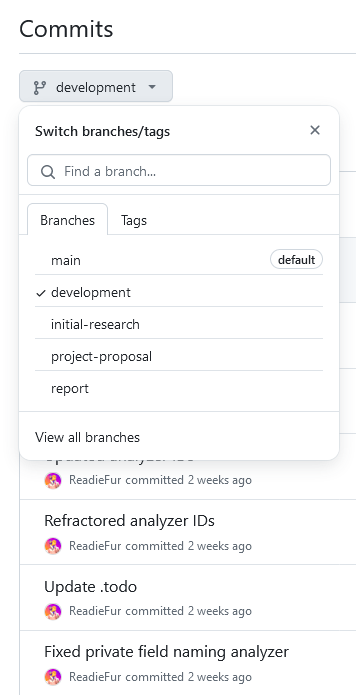
\includegraphics[width=0.25\textwidth]{Figures/GitHubCommitHistoryCropped.png}
% \end{wrapfigure}

When undertaking large projects, it is often recommended to use a project management tool to help keep track of the progress and changes made to the project. Throughout the development lifecycle of this project GitHub was used extensively to track changes and issues (see figure \ref{fig:GitCommitHistory}). GitHub is a web-based platform that uses the Git version control system to track changes made to a project. For this project in particular it allowed for updating existing features with new experiential approaches without the risk of making permanent breaking changes to the existing code. This is because branches can be created via Git that are separate from the main tree and roll back changes if necessary. This is a useful feature as it allows for the project to be developed in a more agile way, where changes can be made quickly and easily without the risk of having to spend time reintegrating old code if the experimental branches do not work out.
